\documentclass[tikz,border=6pt]{standalone}
\usepackage{xcolor}
\usetikzlibrary{arrows.meta,decorations.pathmorphing,calc,positioning,fit,backgrounds,shapes.geometric}
\definecolor{red}{HTML}{A50F2D}\definecolor{ink}{HTML}{141414}\definecolor{gry}{HTML}{5F5F5F}\definecolor{lgry}{HTML}{E6E6E6}
\definecolor{blu}{HTML}{2B6CB0}\definecolor{teal}{HTML}{1B9E8F}\definecolor{org}{HTML}{E8702A}\definecolor{grn}{HTML}{2E9E5B}\definecolor{mag}{HTML}{D81B60}\definecolor{pur}{HTML}{5B2C83}
\tikzset{fibre/.style={ink,line width=1.6pt,line cap=round},
 sis1/.style={org,line width=1.8pt,line cap=round},sis2/.style={blu,line width=1.8pt,line cap=round},
 lab/.style={font=\sffamily\small,text=ink},lbl/.style={font=\sffamily\footnotesize,text=gry,align=center},ttl/.style={font=\sffamily\bfseries\small,text=ink},
 ctcf/.style={-{Triangle[length=5pt,width=6pt]},pur,line width=2.4pt},
 cohesin/.style={grn,line width=1.6pt}}

% ---- shared drawing macros: a DNA duplex is a dark tube with a light core
\newcommand{\dx}[2][ink]{\draw[line width=3.6pt,#1,line cap=round] #2; \draw[line width=1.3pt,white,line cap=round] #2;}
% omega-shaped loop: base at (x,y), radius r
\newcommand{\omegapath}[3]{(#1-0.35,#2) .. controls (#1-0.35,#2+0.45) and (#1-#3,#2+0.35) .. (#1-#3,#2+#3+0.45) arc[start angle=180,end angle=0,radius=#3] .. controls (#1+#3,#2+0.35) and (#1+0.35,#2+0.45) .. (#1+0.35,#2)}
% replication eye: origin at (x,y), half width w, half height h
\newcommand{\eyetop}[4]{(#1-#3,#2) .. controls (#1-#3*0.5,#2+#4*1.33) and (#1+#3*0.5,#2+#4*1.33) .. (#1+#3,#2)}
\newcommand{\eyebot}[4]{(#1-#3,#2) .. controls (#1-#3*0.5,#2-#4*1.33) and (#1+#3*0.5,#2-#4*1.33) .. (#1+#3,#2)}
\newcommand{\eye}[4]{\dx[org]{\eyetop{#1}{#2}{#3}{#4}}\dx[blu]{\eyebot{#1}{#2}{#3}{#4}}\fill[teal] (#1-#3,#2) circle (3.2pt) (#1+#3,#2) circle (3.2pt);}
\newcommand{\ring}[3]{\draw[grn,line width=1.8pt] (#1,#2) ellipse (#3 and #3*1.35);}
\newcommand{\gseg}[3]{\dx[gry]{(#2,#1) -- (#3,#1)}}

\begin{document}
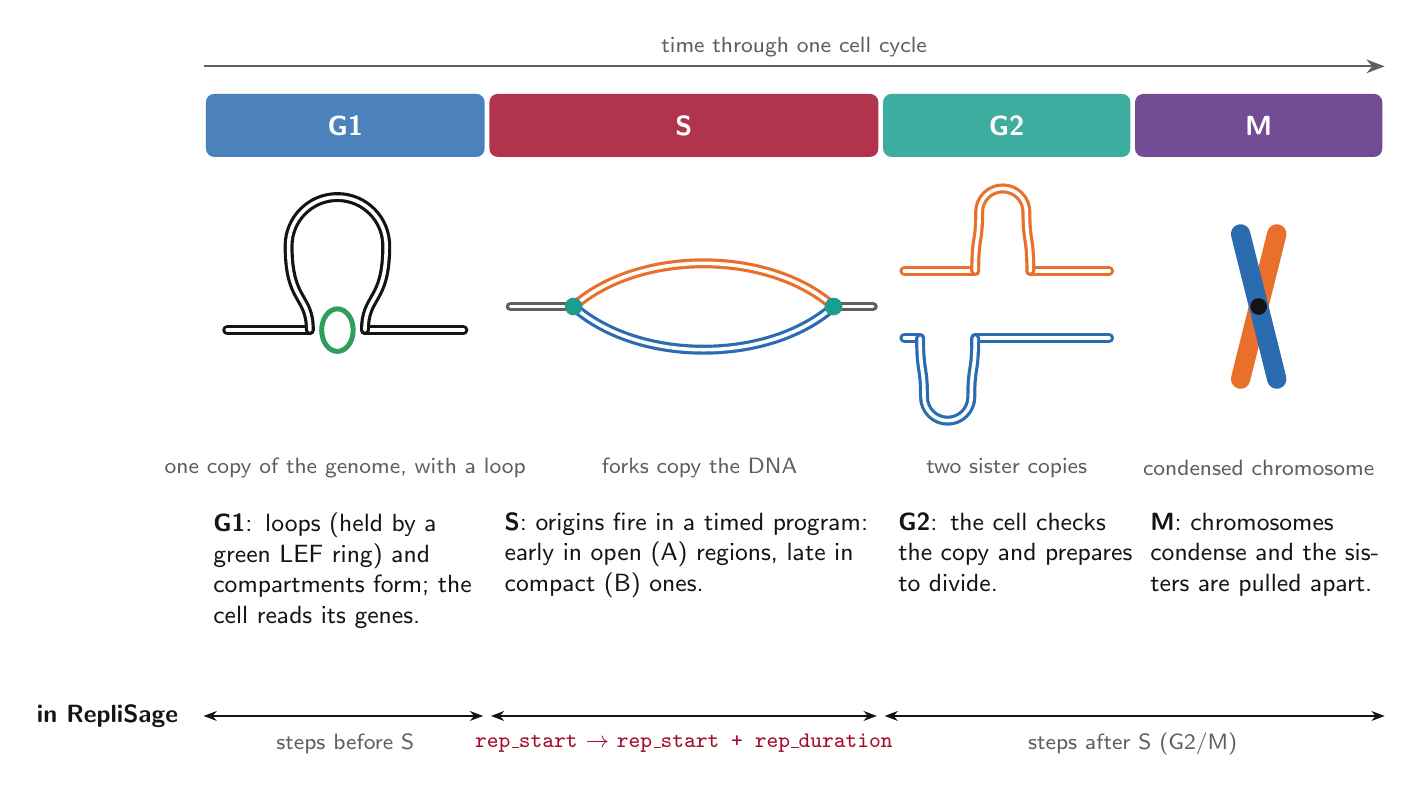
\begin{tikzpicture}[font=\sffamily\small,>=Stealth]
\foreach \x/\w/\c/\t in {0/3.6/blu/{G1},3.6/5.0/red/{S},8.6/3.2/teal/{G2},11.8/3.2/pur/{M}}{
  \fill[\c!85,rounded corners=3pt] (\x+0.03,0) rectangle (\x+\w-0.03,0.8); \node[white,font=\sffamily\bfseries] at (\x+\w/2,0.4) {\t};}
\draw[->,gry,thick] (0,1.15) -- (15,1.15); \node[lbl,anchor=south] at (7.5,1.15) {time through one cell cycle};
\begin{scope}[yshift=-2.2cm]
 % G1: one fibre with a loop and a cohesin ring
 \dx{(0.3,0) -- (1.35,0)} \dx{(2.05,0) -- (3.3,0)} \dx{\omegapath{1.7}{0}{0.62}} \ring{1.7}{0}{0.2}
 % S: one replication eye
 \dx[gry]{(3.9,0.3) -- (4.7,0.3)} \dx[gry]{(8.0,0.3) -- (8.5,0.3)}
 \eye{6.35}{0.3}{1.65}{0.55}
 % G2: two sister copies side by side, each with its own loops
\dx[org]{(8.9,0.75) -- (9.8,0.75)} \dx[org]{(10.5,0.75) -- (11.5,0.75)} \begin{scope}[shift={(0,0.75)}] \dx[org]{\omegapath{10.15}{0}{0.3}} \end{scope}
\dx[blu]{(8.9,-0.1) -- (9.1,-0.1)} \dx[blu]{(9.8,-0.1) -- (11.5,-0.1)} \begin{scope}[shift={(9.45,-0.1)},rotate=180] \dx[blu]{\omegapath{0}{0}{0.3}} \end{scope}
 % M: condensed chromosome (X shape: two sisters joined at the centromere)
 \begin{scope}[shift={(13.4,0.3)}]
  \draw[org,line width=7pt,line cap=round,rotate=-14] (0,-0.95) -- (0,0.95);
  \draw[blu,line width=7pt,line cap=round,rotate=14] (0,-0.95) -- (0,0.95);
  \fill[ink] (0,0) circle (3pt);
 \end{scope}
\end{scope}
\node[lbl] at (1.8,-3.95) {one copy of the genome, with a loop};
\node[lbl] at (6.3,-3.95) {forks copy the DNA};
\node[lbl] at (10.2,-3.95) {two sister copies};
\node[lbl] at (13.4,-3.95) {condensed chromosome};
\node[lab,align=left,anchor=north west,text width=3.4cm] at (0,-4.4) {\textbf{G1}: loops (held by a green LEF ring) and compartments form; the cell reads its genes.};
\node[lab,align=left,anchor=north west,text width=4.8cm] at (3.7,-4.4) {\textbf{S}: origins fire in a timed program: early in open (A) regions, late in compact (B) ones.};
\node[lab,align=left,anchor=north west,text width=3.0cm] at (8.7,-4.4) {\textbf{G2}: the cell checks the copy and prepares to divide.};
\node[lab,align=left,anchor=north west,text width=3.0cm] at (11.9,-4.4) {\textbf{M}: chromosomes condense and the sisters are pulled apart.};
\draw[<->,ink] (0,-7.1) -- (3.55,-7.1); \draw[<->,ink] (3.65,-7.1) -- (8.55,-7.1); \draw[<->,ink] (8.65,-7.1) -- (15,-7.1);
\node[lbl] at (1.8,-7.45) {steps before S}; \node[lbl,red] at (6.1,-7.45) {\texttt{rep\_start} $\to$ \texttt{rep\_start + rep\_duration}}; \node[lbl] at (11.8,-7.45) {steps after S (G2/M)};
\node[ttl,anchor=east] at (-0.2,-7.1) {in RepliSage};
\end{tikzpicture}
\end{document}
